\begin{figure}[H]
	\centering
	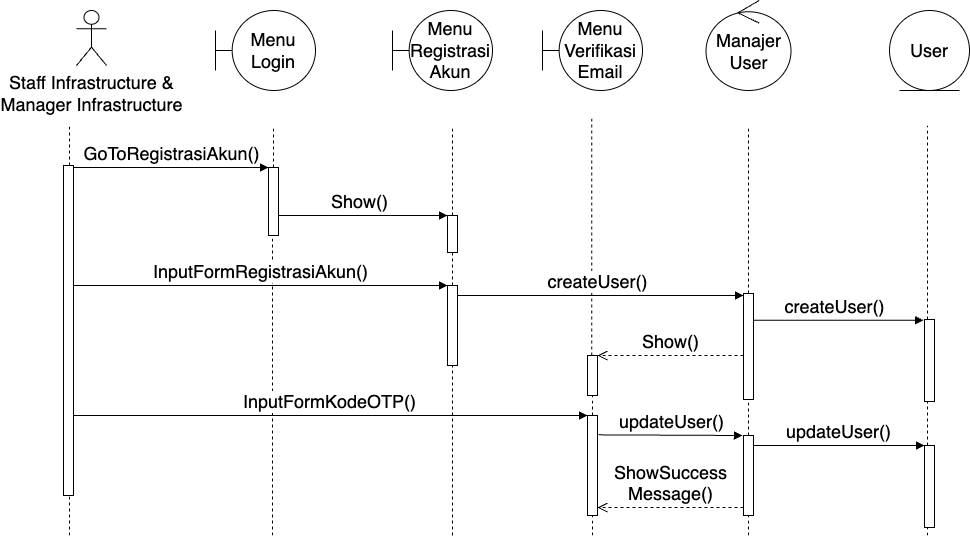
\includegraphics[width=15cm]{Gambar/bab2/sequence-diagram-registrasi-akun.png}
	\caption{\textit{Sequence Diagram} Registrasi Akun}
	\label{fig:sequence-diagram-registrasi-akun}
\end{figure}
\FloatBarrier

\begin{figure}[H]
	\centering
	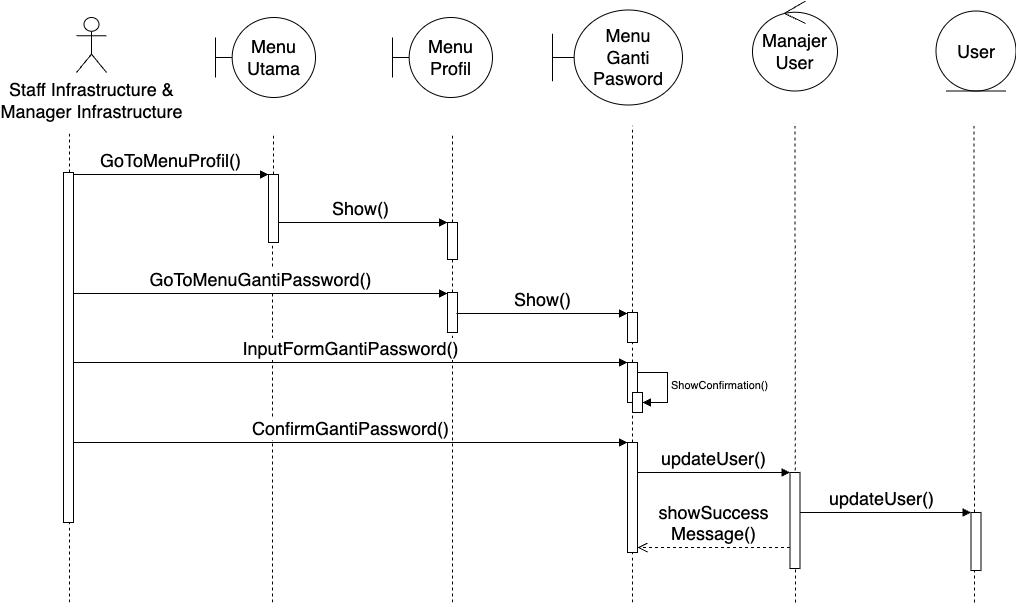
\includegraphics[width=15cm]{Gambar/bab2/sequence-diagram-ganti-password.png}
	\caption{\textit{Sequence Diagram} Ganti Password}
	\label{fig:sequence-diagram-ganti-password}
\end{figure}
\FloatBarrier

\begin{figure}[H]
	\centering
	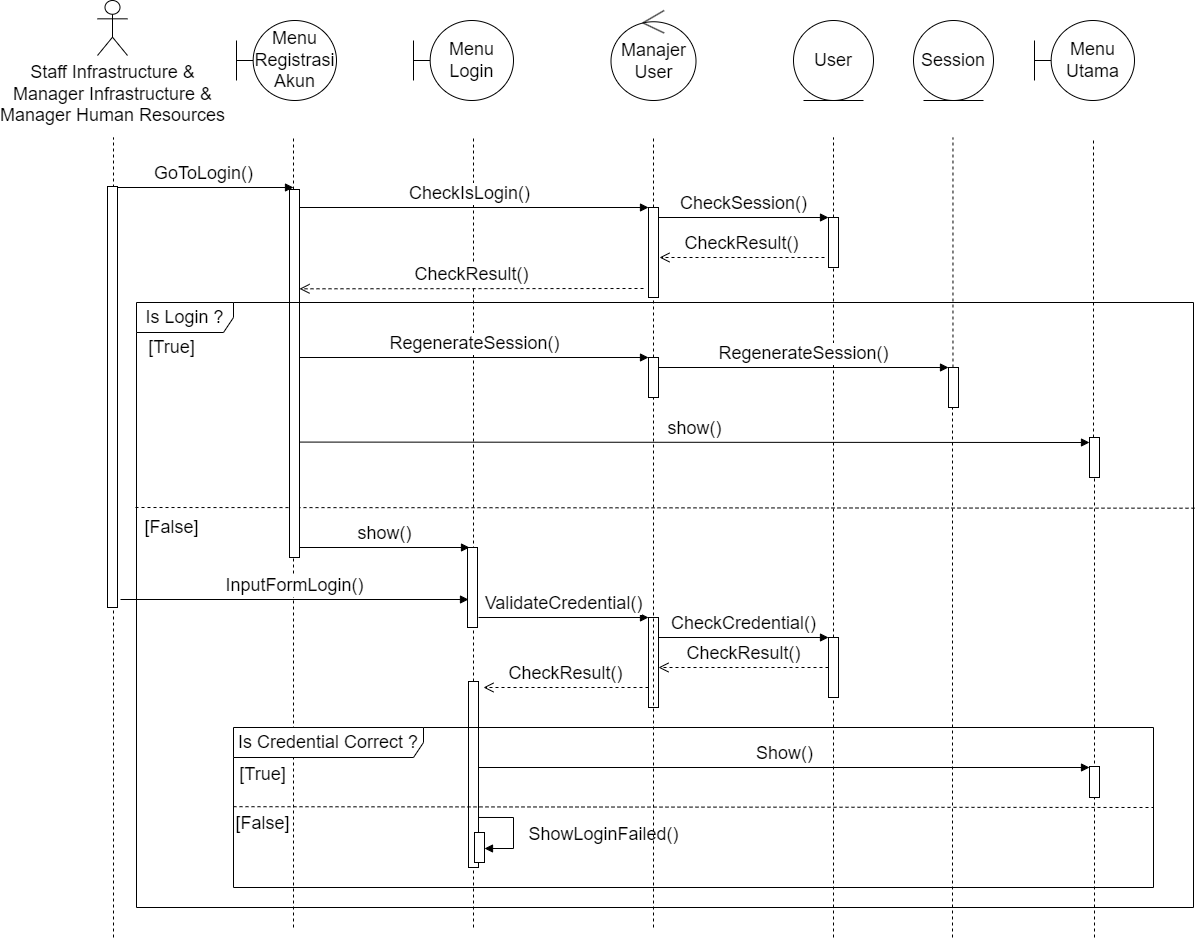
\includegraphics[width=17cm]{Gambar/bab2/sequence-diagram-login.png}
	\caption{\textit{Sequence Diagram Login}}
	\label{fig:sequence-diagram-login}
\end{figure}
\FloatBarrier

\begin{figure}[H]
	\centering
	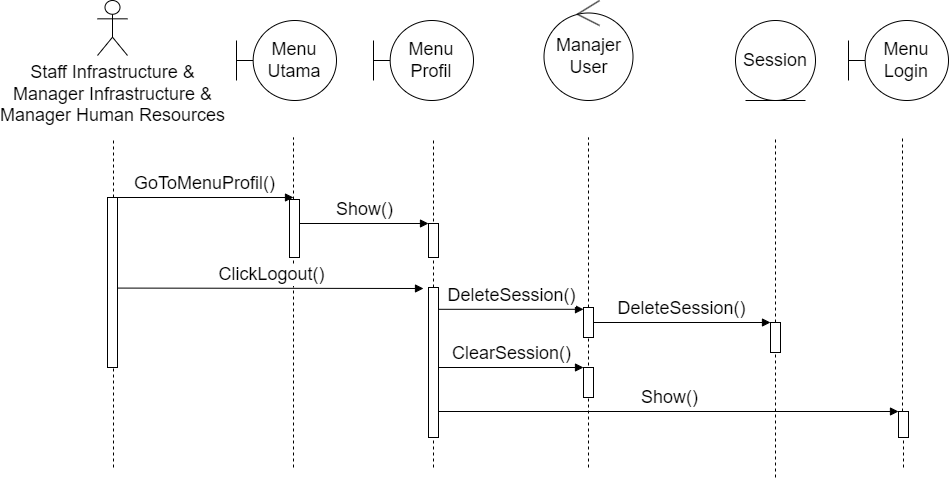
\includegraphics[width=17cm]{Gambar/bab2/sequence-diagram-logout.png}
	\caption{\textit{Sequence Diagram Logout}}
	\label{fig:sequence-diagram-logout}
\end{figure}
\FloatBarrier

\begin{figure}[H]
	\centering
	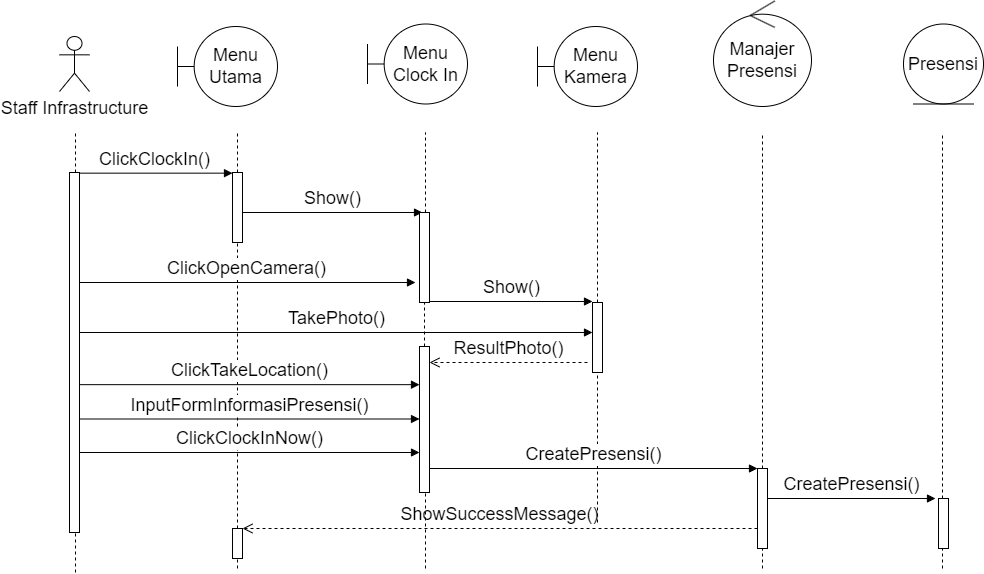
\includegraphics[width=17cm]{Gambar/bab2/sequence-diagram-clock-in.png}
	\caption{\textit{Sequence Diagram Clock In}}
	\label{fig:sequence-diagram-clock-in}
\end{figure}
\FloatBarrier

\begin{figure}[H]
	\centering
	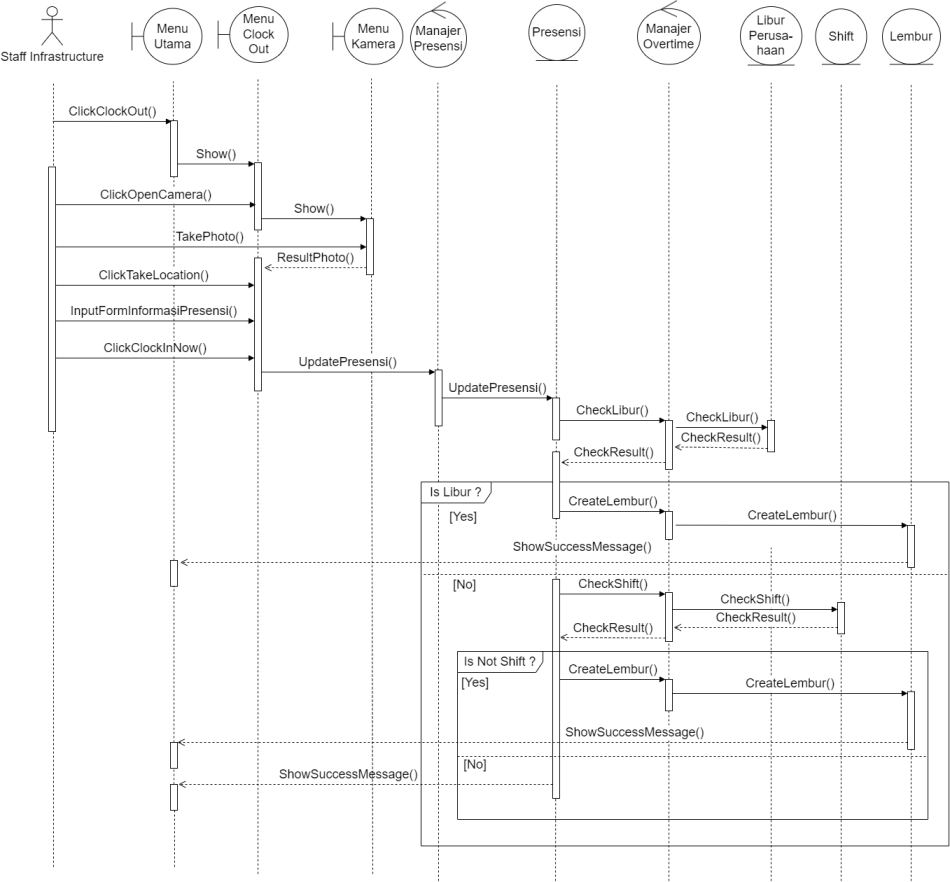
\includegraphics[width=18cm]{Gambar/bab2/sequence-diagram-clock-out.png}
	\caption{\textit{Sequence Diagram Clock Out}}
	\label{fig:sequence-diagram-clock-out}
\end{figure}
\FloatBarrier

\begin{figure}[H]
	\centering
	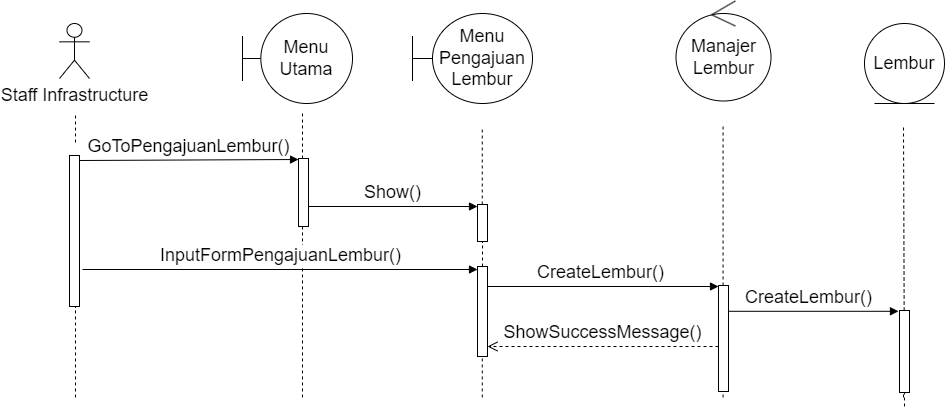
\includegraphics[width=17cm]{Gambar/bab2/sequence-diagram-melakukan-pengajuan-lembur.png}
	\caption{\textit{Sequence Diagram} Melakukan Pengajuan Lembur}
	\label{fig:sequence-diagram-melakukan-pengajuan-lembur}
\end{figure}
\FloatBarrier

\begin{figure}[H]
	\centering
	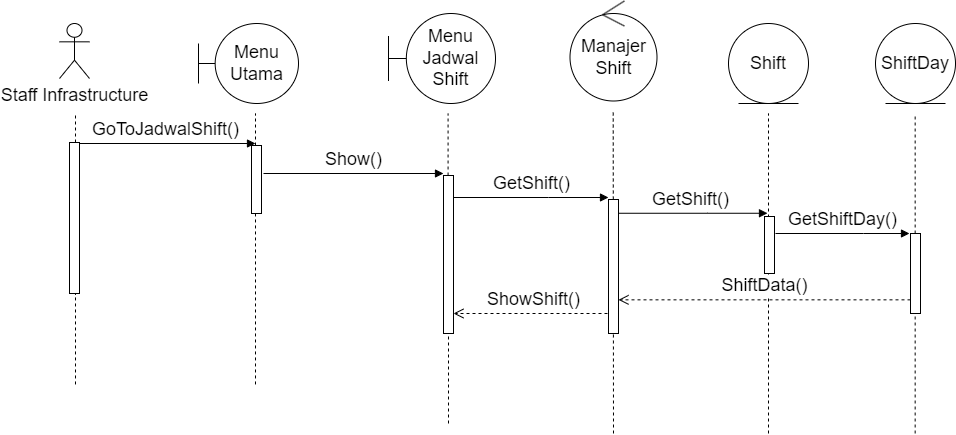
\includegraphics[width=17cm]{Gambar/bab2/sequence-diagram-melihat-jadwal-shift.png}
	\caption{\textit{Sequence Diagram} Melihat Jadwal \textit{Shift} Kerja}
	\label{fig:sequence-diagram-melihat-jadwal-shift-kerja}
\end{figure}
\FloatBarrier

\begin{figure}[H]
	\centering
	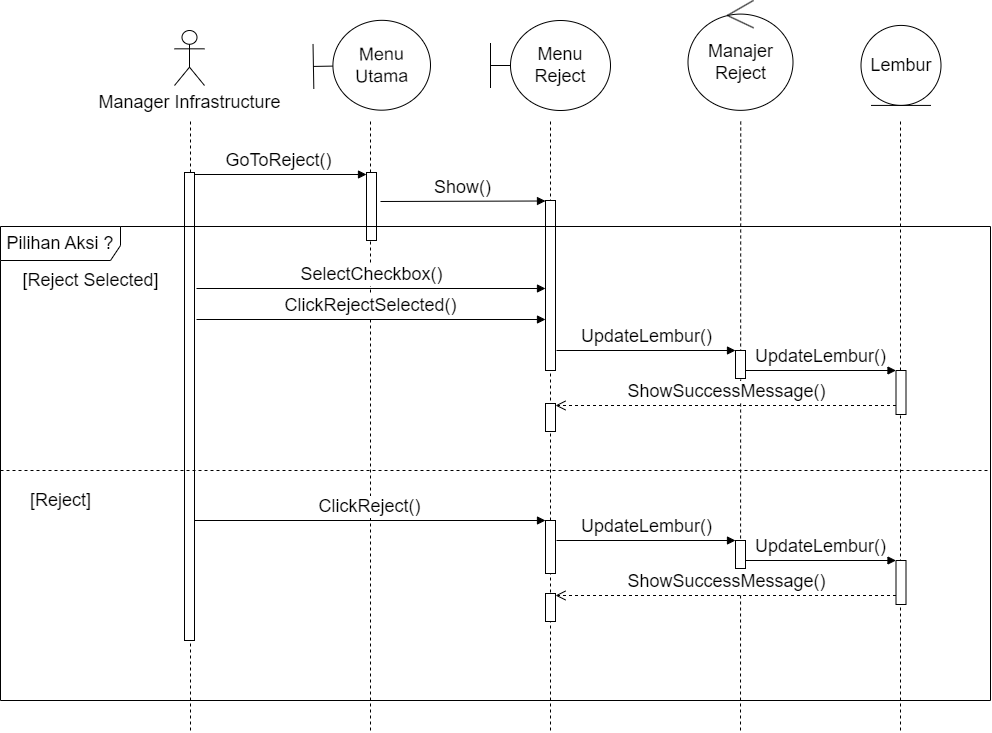
\includegraphics[width=17cm]{Gambar/bab2/sequence-diagram-melakukan-reject.png}
	\caption{\textit{Sequence Diagram} Melakukan \textit{Reject} pada Data Lembur}
	\label{fig:sequence-diagram-melakukan-reject-pada-data-lembur}
\end{figure}
\FloatBarrier

\begin{figure}[H]
	\centering
	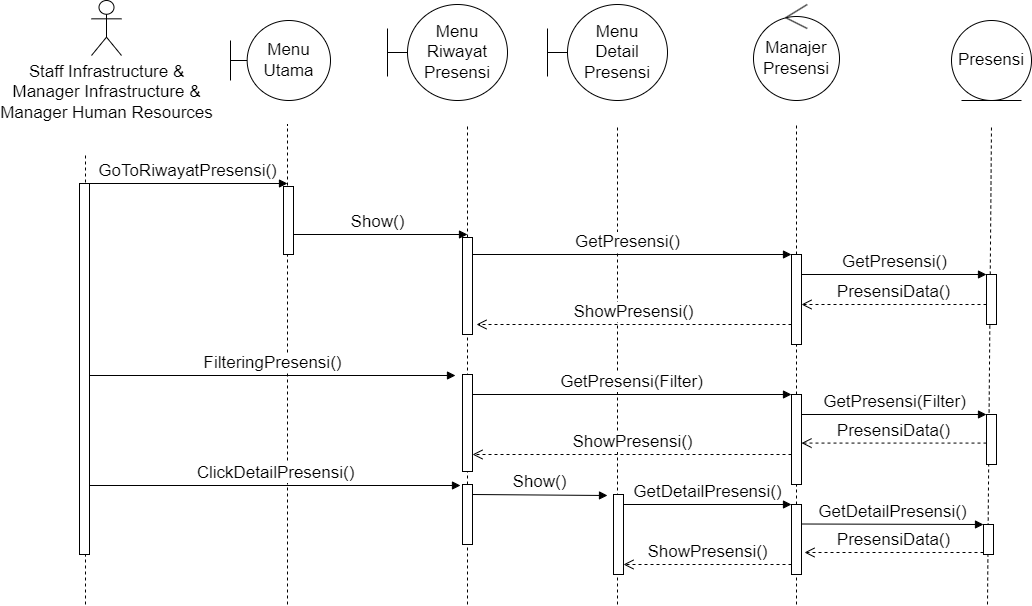
\includegraphics[width=17cm]{Gambar/bab2/sequence-diagram-melihat-riwayat-presensi.png}
	\caption{\textit{Sequence Diagram} Melihat Riwayat Presensi}
	\label{fig:sequence-diagram-melihat-riwayat-presensi}
\end{figure}
\FloatBarrier

\begin{figure}[H]
	\centering
	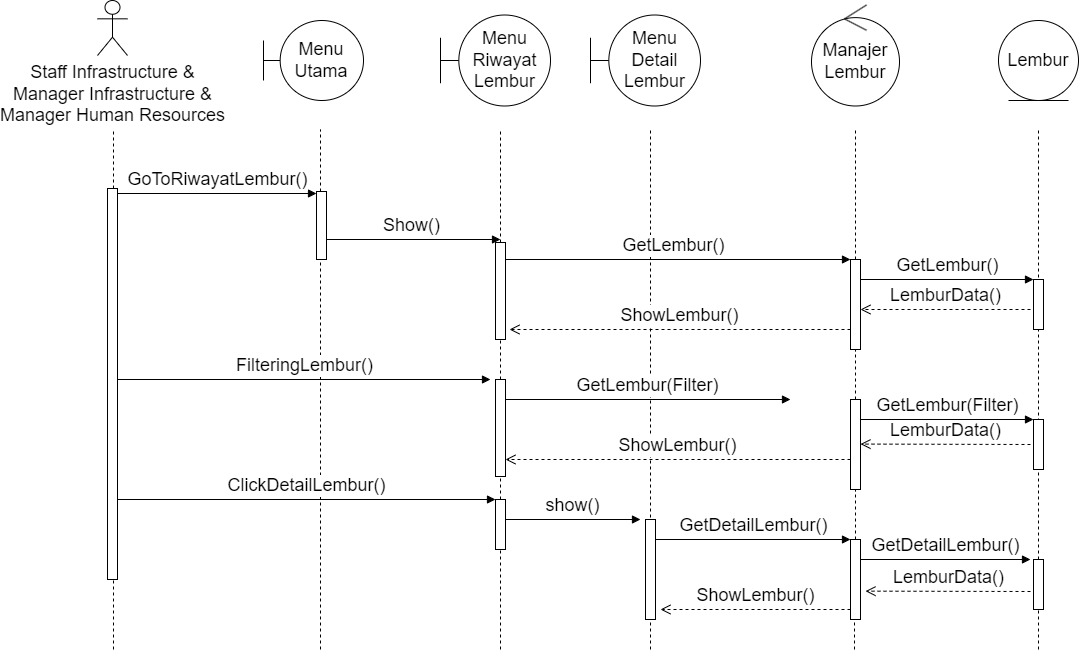
\includegraphics[width=17cm]{Gambar/bab2/sequence-diagram-melihat-riwayat-lembur.png}
	\caption{\textit{Sequence Diagram} Melihat Riwayat Lembur}
	\label{fig:sequence-diagram-melihat-riwayat-lembur}
\end{figure}
\FloatBarrier

\begin{figure}[H]
	\centering
	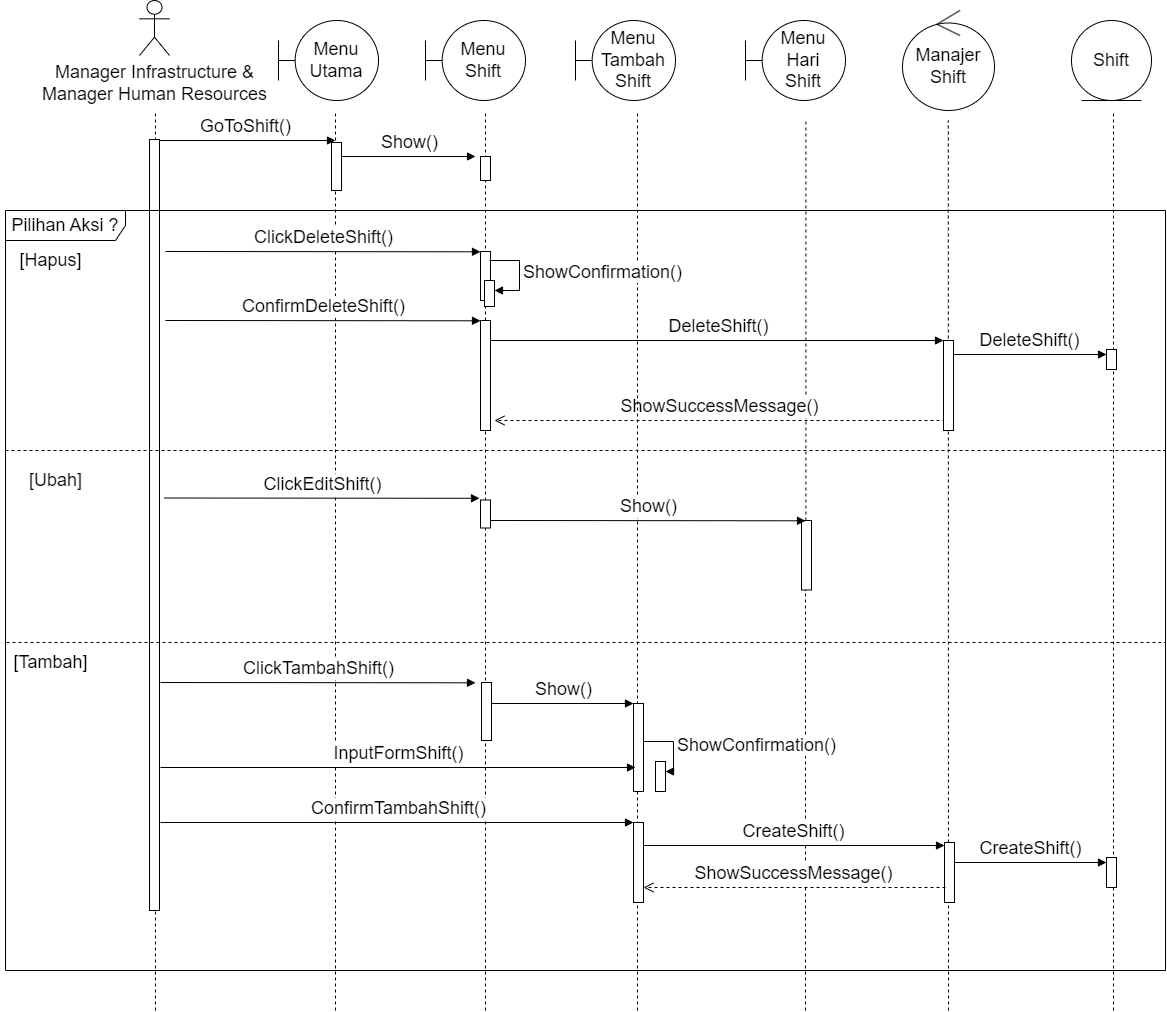
\includegraphics[width=18cm]{Gambar/bab2/sequence-diagram-mengelola-data-jenis-shift.png}
	\caption{\textit{Sequence Diagram} Mengelola Jenis \textit{Shift}}
	\label{fig:sequence-diagram-mengelola-jenis-shift}
\end{figure}
\FloatBarrier

\begin{figure}[H]
	\centering
	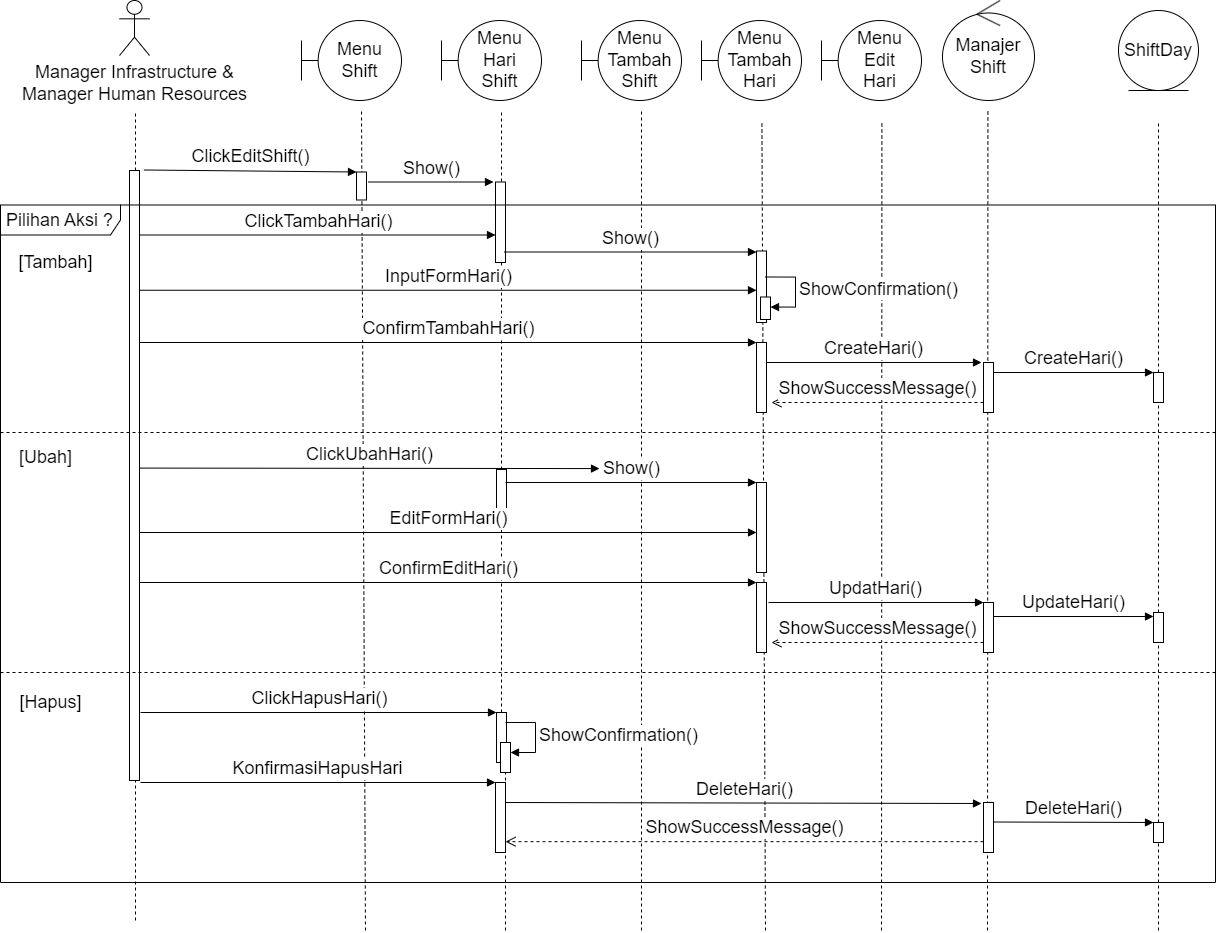
\includegraphics[width=18cm]{Gambar/bab2/sequence-diagram-mengelola-data-hari-shift.png}
	\caption{\textit{Sequence Diagram} Mengelola Hari \textit{Shift}}
	\label{fig:sequence-diagram-mengelola-hari-shift}
\end{figure}
\FloatBarrier

\begin{figure}[H]
	\centering
	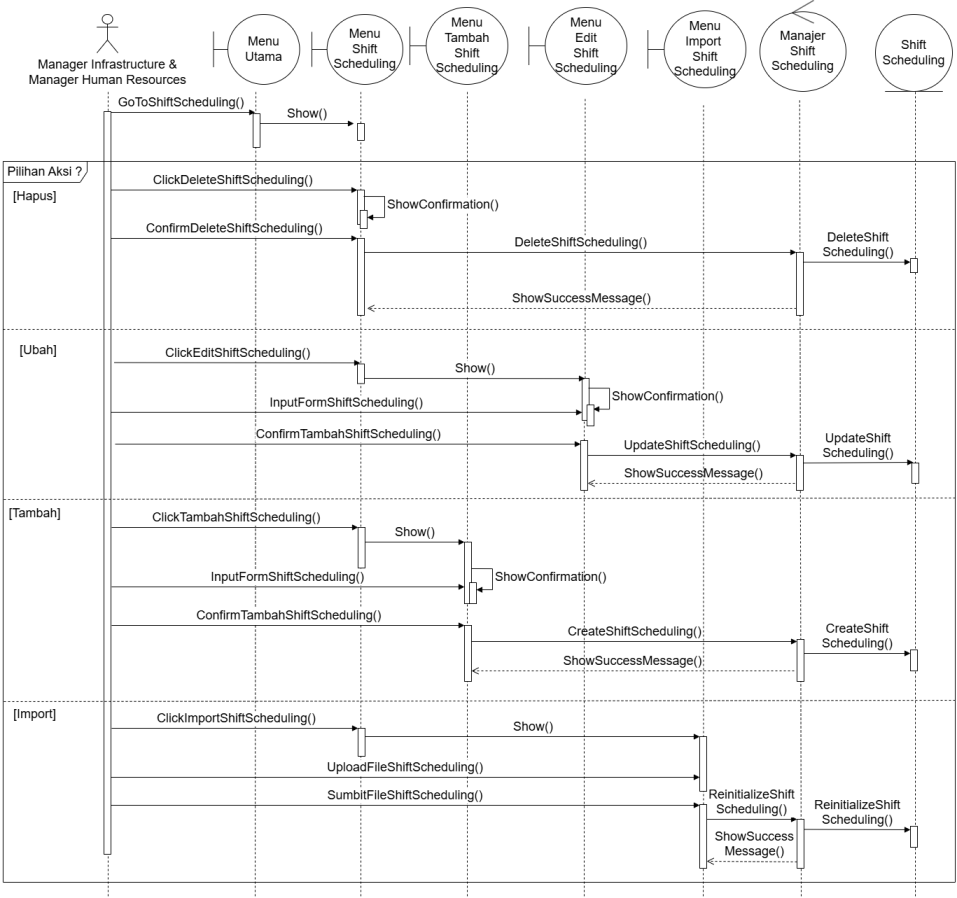
\includegraphics[width=18cm]{Gambar/bab2/sequence-diagram-mengelola-data-penjadwalan-shift.png}
	\caption{\textit{Sequence Diagram} Mengelola Penjadwalan \textit{Shift}}
	\label{fig:sequence-diagram-mengelola-penjadwalan-shift}
\end{figure}
\FloatBarrier

\begin{figure}[H]
	\centering
	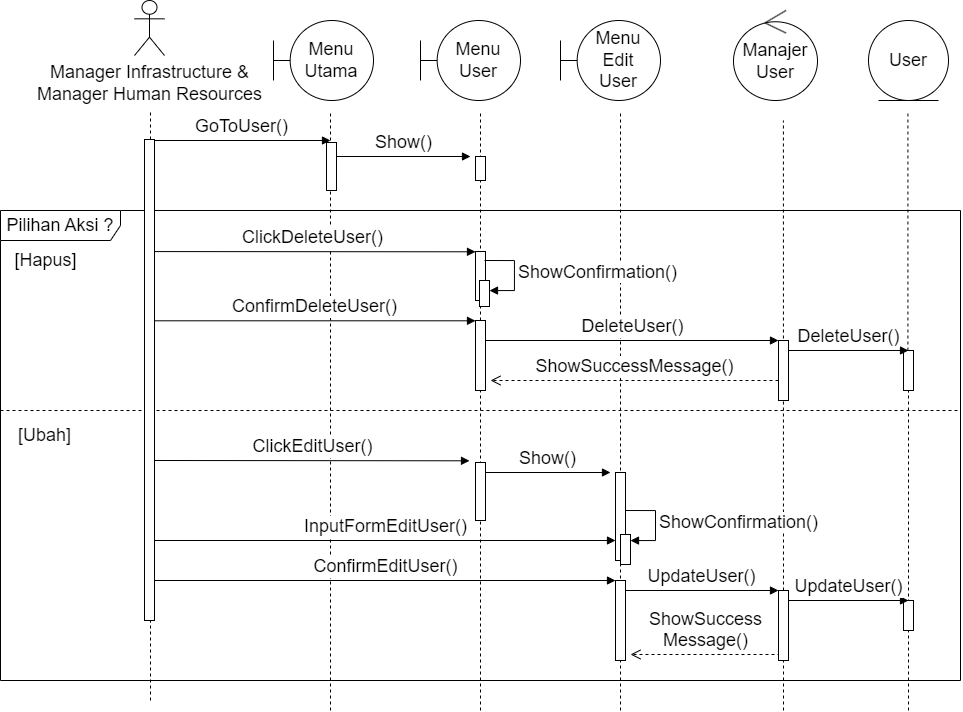
\includegraphics[width=15cm]{Gambar/bab2/sequence-diagram-mengelola-akun-user.png}
	\caption{\textit{Sequence Diagram} Mengelola Akun \textit{User}}
	\label{fig:sequence-diagram-mengelola-akun-user}
\end{figure}
\FloatBarrier

\begin{figure}[H]
	\centering
	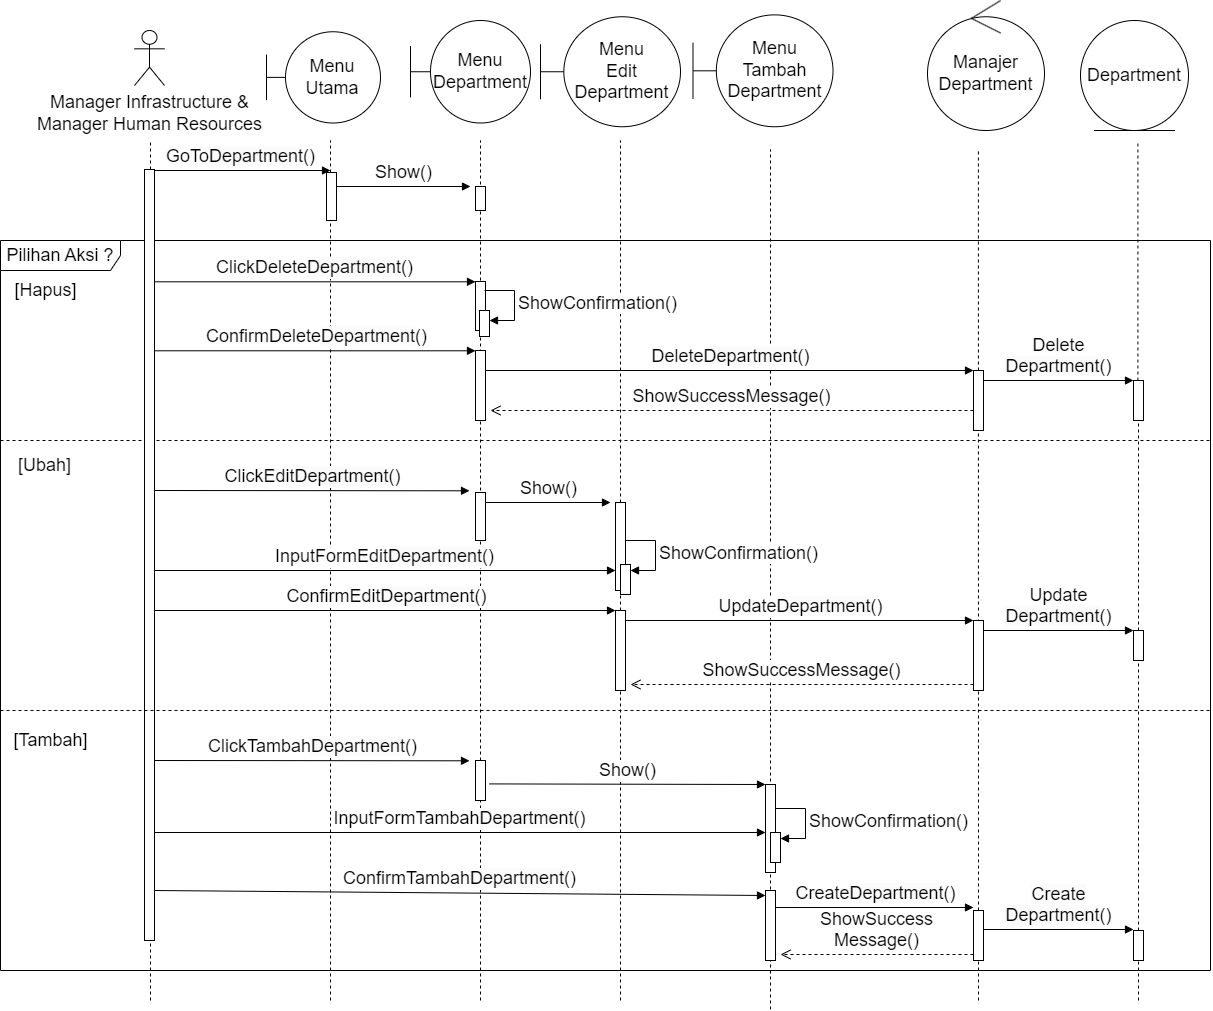
\includegraphics[width=15cm]{Gambar/bab2/sequence-diagram-mengelola-department.png}
	\caption{\textit{Sequence Diagram} Mengelola \textit{Department}}
	\label{fig:sequence-diagram-mengelola-department}
\end{figure}
\FloatBarrier

\begin{figure}[H]
	\centering
	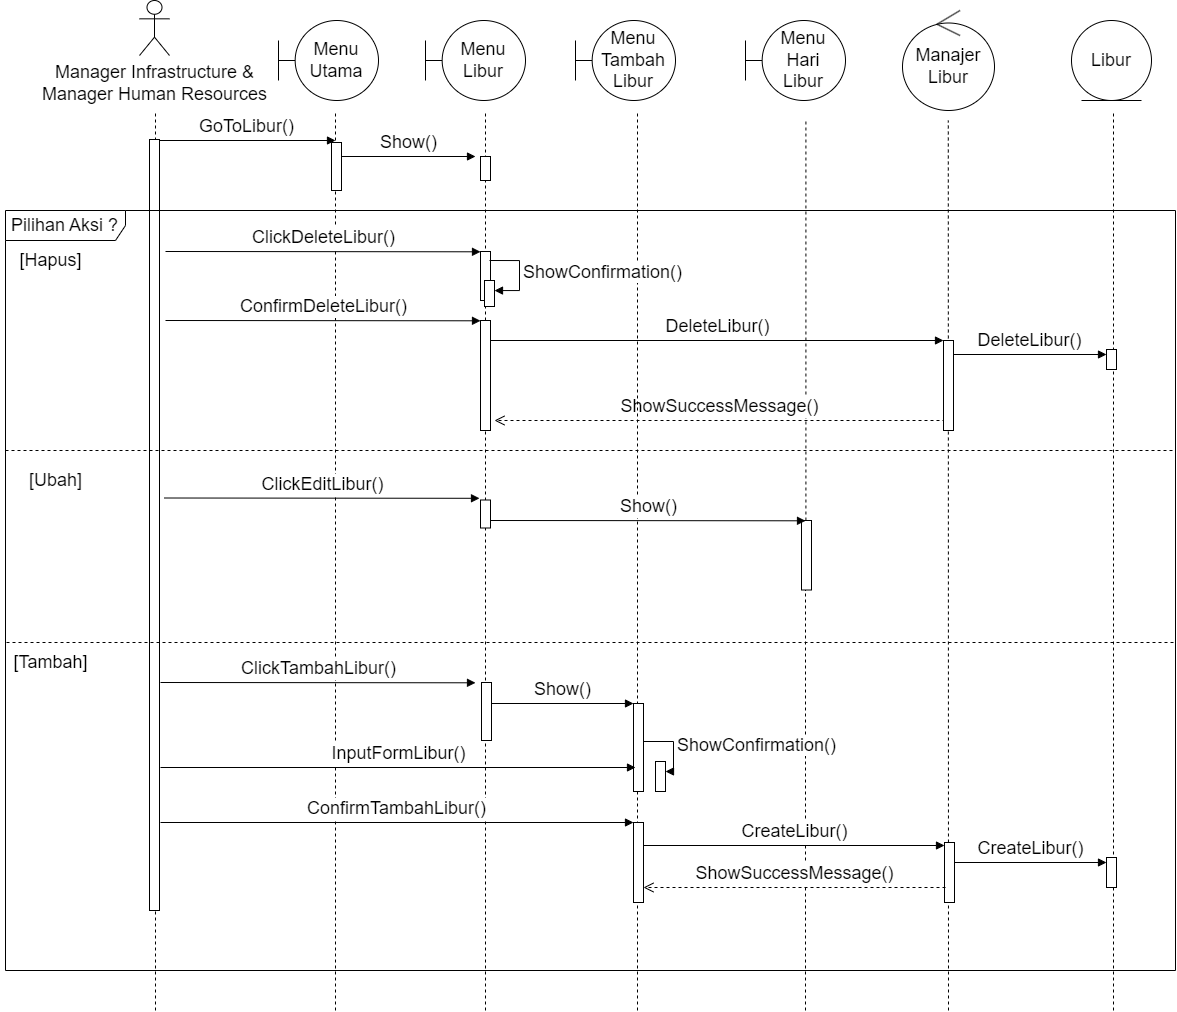
\includegraphics[width=15cm]{Gambar/bab2/sequence-diagram-mengelola-data-jenis-libur.png}
	\caption{\textit{Sequence Diagram} Mengelola Data Jenis Libur Perusahaan}
	\label{fig:sequence-diagram-mengelola-data-jenis-libur-perusahaan}
\end{figure}
\FloatBarrier

\begin{figure}[H]
	\centering
	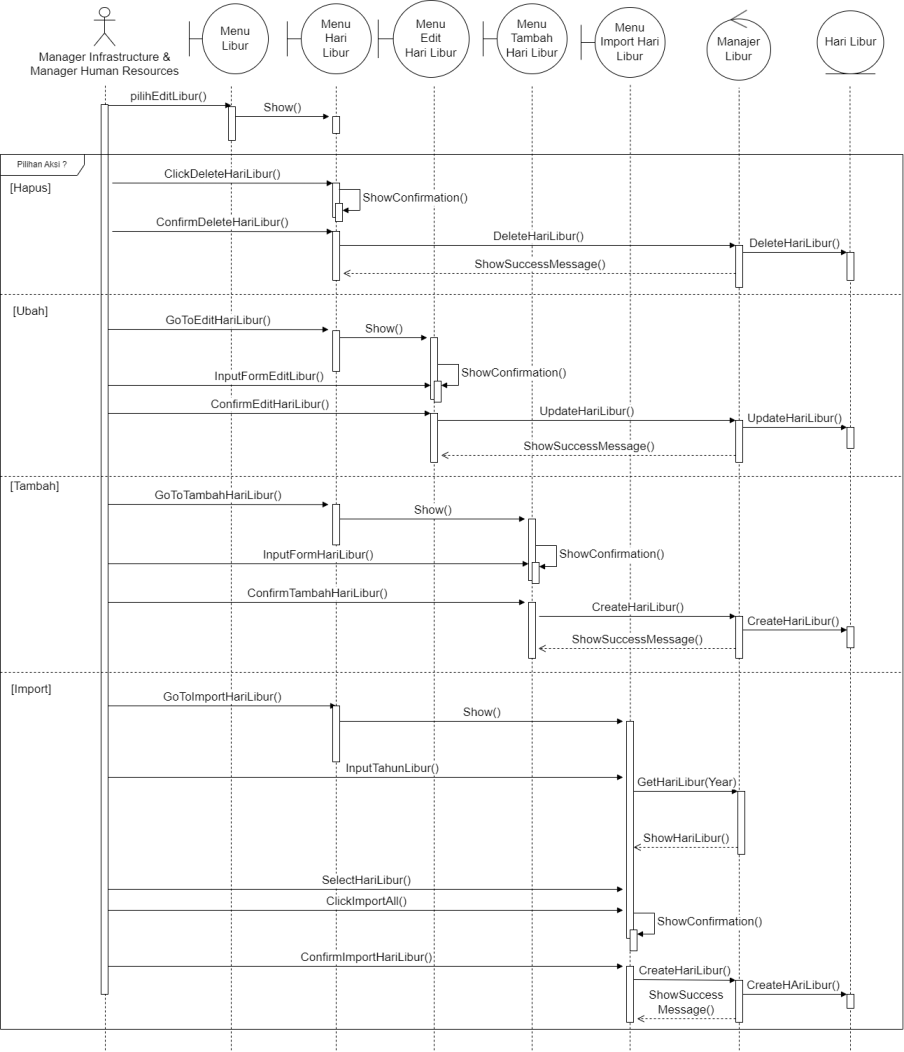
\includegraphics[width=15cm]{Gambar/bab2/sequence-diagram-mengelola-data-hari-libur.png}
	\caption{\textit{Sequence Diagram} Mengelola Data Hari Libur Perusahaan}
	\label{fig:sequence-diagram-mengelola-data-hari-libur-perusahaan}
\end{figure}
\FloatBarrier

\begin{figure}[H]
	\centering
	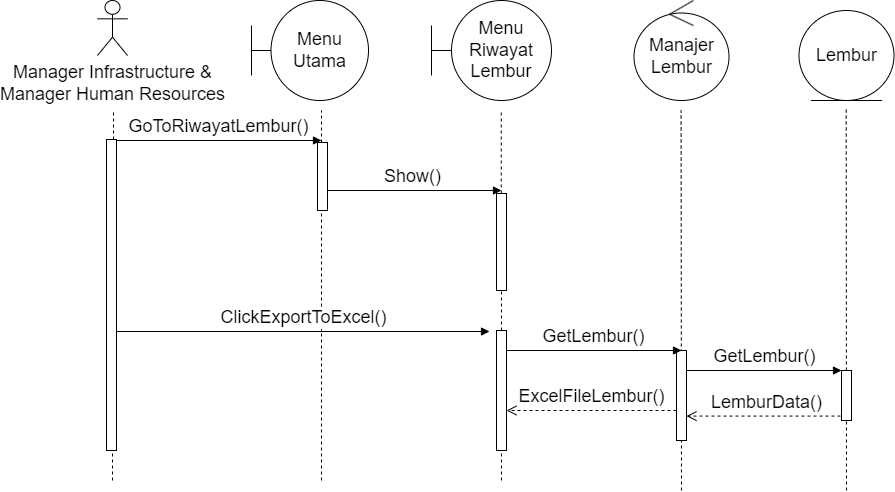
\includegraphics[width=15cm]{Gambar/bab2/sequence-diagram-melakukan-export-data-lembur-ke-excel.png}
	\caption{\textit{Sequence Diagram} melakukan \textit{Export} Data Lembur ke \textit{Excel}}
	\label{fig:sequence-diagram-melakukan-export-data-lembur-ke-excel}
\end{figure}
\FloatBarrier

\begin{figure}[H]
	\centering
	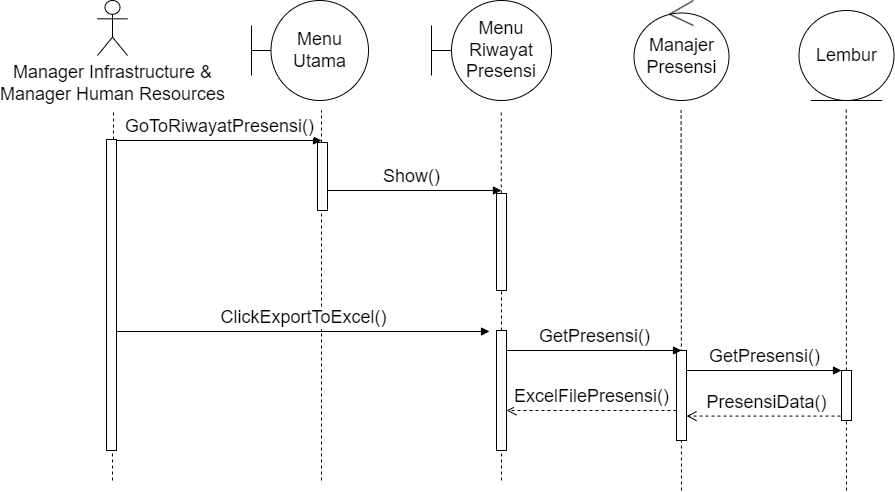
\includegraphics[width=15cm]{Gambar/bab2/sequence-diagram-melakukan-export-data-presensi-ke-excel.png}
	\caption{\textit{Sequence Diagram} melakukan \textit{Export} Data Presensi ke \textit{Excel}}
	\label{fig:sequence-diagram-melakukan-export-data-presensi-ke-excel}
\end{figure}
\FloatBarrier